\documentclass{beamer}

%\usepackage[table]{xcolor}
\mode<presentation> {
  \usetheme{Boadilla}
%  \usetheme{Pittsburgh}
%\usefonttheme[2]{sans}
\renewcommand{\familydefault}{cmss}
%\usepackage{lmodern}
%\usepackage[T1]{fontenc}
%\usepackage{palatino}
%\usepackage{cmbright}

\useinnertheme{rectangles}
}
%\usepackage{normalem}{ulem}
%\usepackage{colortbl, textcomp}
\setbeamercolor{normal text}{fg = black}
\setbeamercolor{structure}{fg = blue}
\definecolor{trial}{cmyk}{1,0,0, 0}
\definecolor{trial2}{cmyk}{0.00,0,1, 0}
\definecolor{darkgreen}{rgb}{0,.4, 0.1}
\definecolor{mygray}{gray}{0.8}
\definecolor{myblack}{rgb}{0, 0, 0}
\usepackage{array}
\beamertemplatesolidbackgroundcolor{white}  \setbeamercolor{alerted
text}{fg=red}

\setbeamertemplate{caption}[numbered]\newcounter{mylastframe}

\usepackage{color}
\usepackage{tikz}
\usetikzlibrary{arrows}
\usepackage{colortbl}
\usepackage{graphicx}
\usepackage{epsfig}

%\usepackage[usenames, dvipsnames]{color}
%\setbeamertemplate{caption}[numbered]\newcounter{mylastframe}c
%\newcolumntype{Y}{\columncolor[cmyk]{0, 0, 1, 0}\raggedright}
%\newcolumntype{C}{\columncolor[cmyk]{1, 0, 0, 0}\raggedright}
%\newcolumntype{G}{\columncolor[rgb]{0, 1, 0}\raggedright}
%\newcolumntype{R}{\columncolor[rgb]{1, 0, 0}\raggedright}

%\begin{beamerboxesrounded}[upper=uppercol,lower=lowercol,shadow=true]{Block}
%$A = B$.
%\end{beamerboxesrounded}}
\renewcommand{\familydefault}{cmss}
%\usepackage[all]{xy}

\usepackage{tikz}
\usepackage{lipsum}

 \newenvironment{changemargin}[3]{%
 \begin{list}{}{%
 \setlength{\topsep}{0pt}%
 \setlength{\leftmargin}{#1}%
 \setlength{\rightmargin}{#2}%
 \setlength{\topmargin}{#3}%
 \setlength{\listparindent}{\parindent}%
 \setlength{\itemindent}{\parindent}%
 \setlength{\parsep}{\parskip}%
 }%
\item[]}{\end{list}}
\usetikzlibrary{arrows}
%\usepackage{palatino}
%\usepackage{eulervm}
\usecolortheme{lily}

\newtheorem{com}{Comment}
\newtheorem{lem} {Lemma}
\newtheorem{prop}{Proposition}
\newtheorem{thm}{Theorem}
\newtheorem{defn}{Definition}
\newtheorem{cor}{Corollary}
\newtheorem{obs}{Observation}
 \numberwithin{equation}{section}


\title[PLSC 43401] % (optional, nur bei langen Titeln nötig)
{Mathematical Foundations of Political Methodology}

\author{Robert Gulotty}
\institute[University of Chicago]{Department of Political Science \\  University of Chicago}
\vspace{0.3in}
\date{}

\setbeamertemplate{navigation symbols}{}

\begin{document}



\begin{frame}
\titlepage
\end{frame}



\begin{frame}
\frametitle{Why Do We Need to Learn Calculus}

\ \\ Calculus is everywhere in the sciences.  Without it, we would not have had the First Industrial Revolution. \pause

\ \\These slides preview and help justify the study of calculus for political scientists.

\end{frame}


\begin{frame}
\frametitle{Example 1: Derivative in Positive Political Economy }
\begin{itemize}
\item The derivative refers to an instantaneous notion of change. \pause
\item The marginalist perspective reframes problems in terms of marginal costs and benefits: why do newspapers dispensers operate differently than candy dispensers?\pause
\item The first newspaper is valuable, the second and third less so.  This is the notion of marginal utility.


\begin{figure}[!htb]
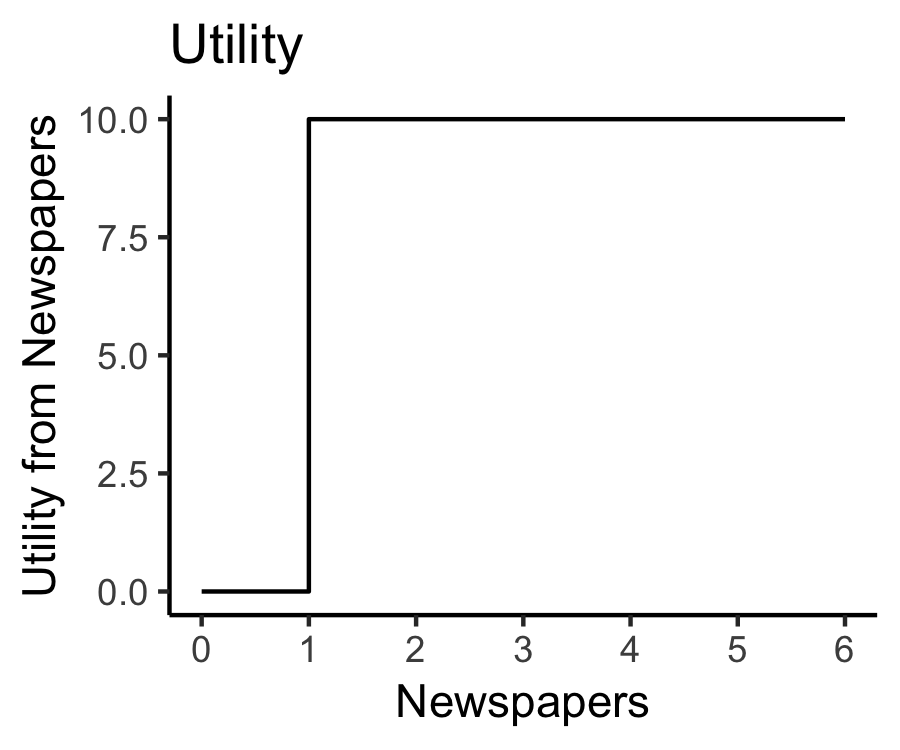
\includegraphics[width=2 in]{p1.png}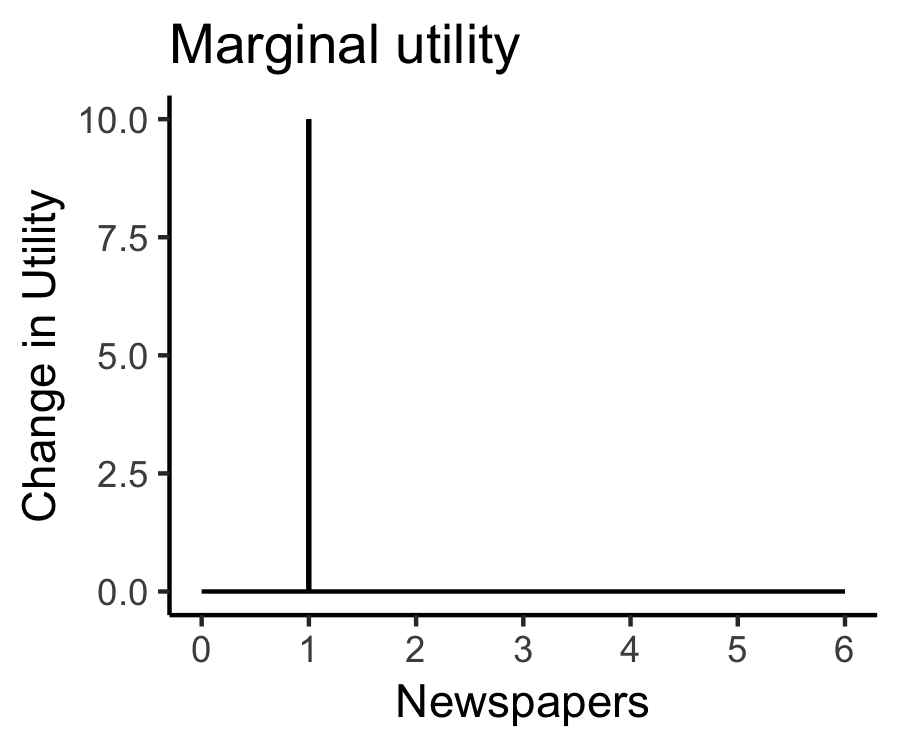
\includegraphics[width=2 in]{p2.png}
\end{figure}
\end{itemize}
\end{frame}

\begin{frame}
\frametitle[plain]{The benefits of being smooth}


\begin{figure}[!htb]
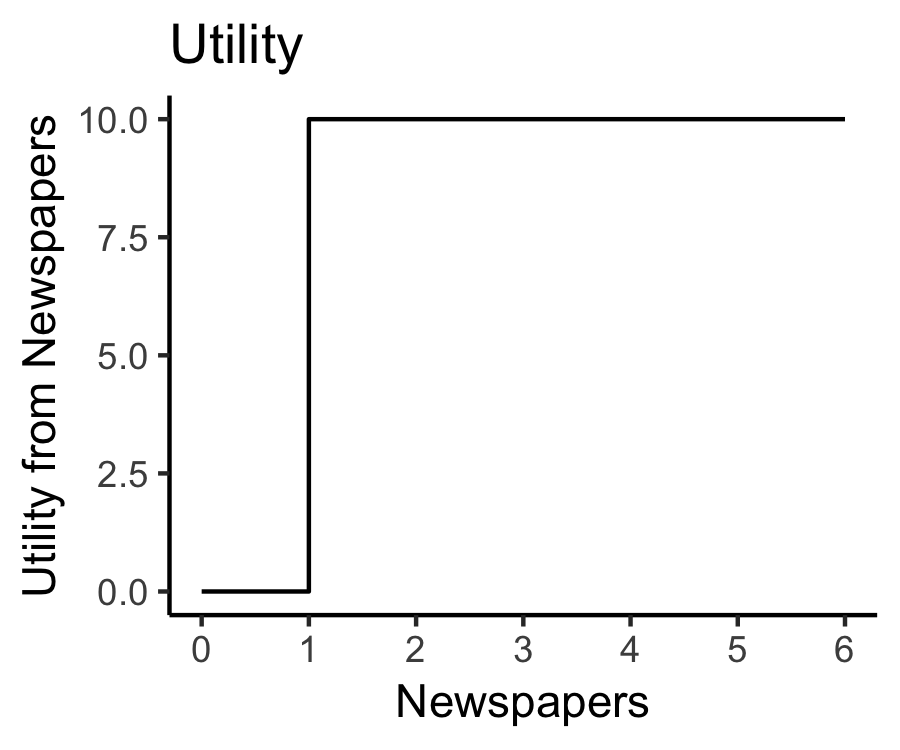
\includegraphics[width=1.8 in]{p1.png}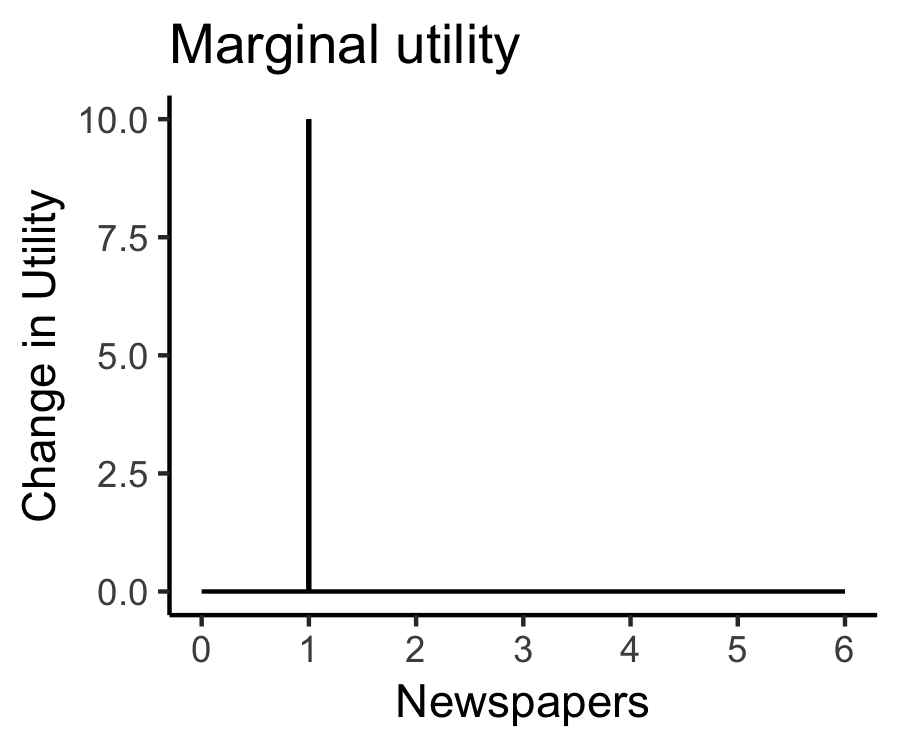
\includegraphics[width=1.8 in]{p2.png}\\\pause
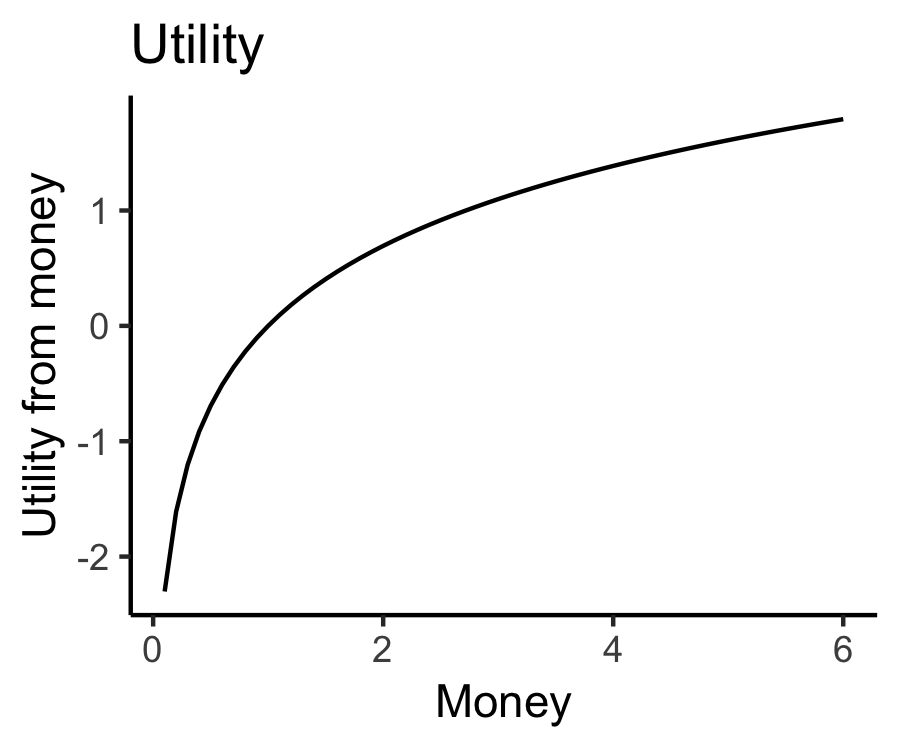
\includegraphics[width=1.8 in]{p3.png}\pause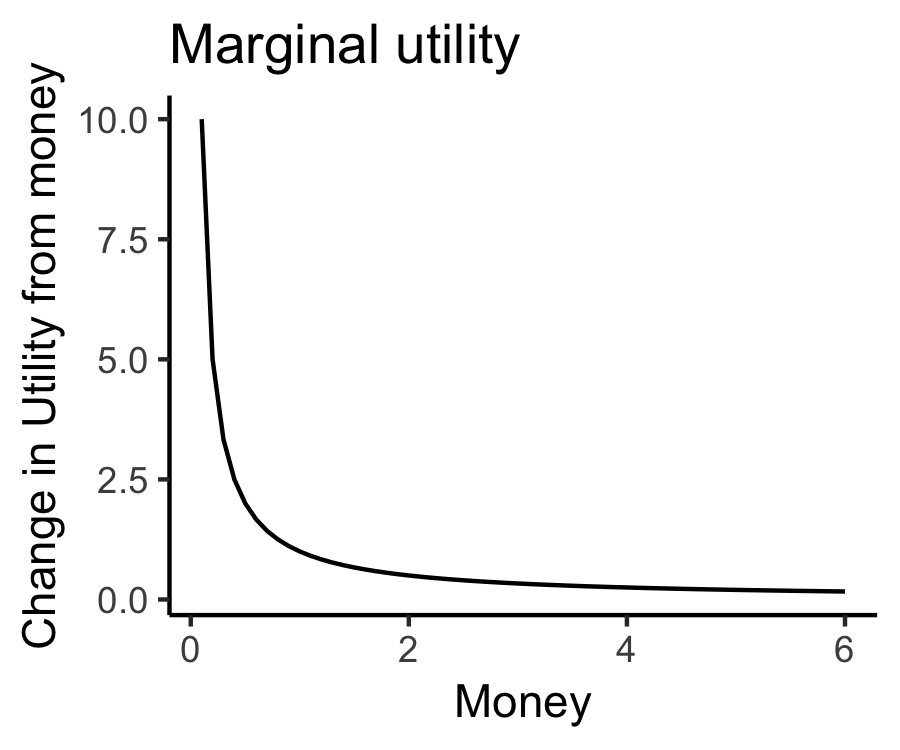
\includegraphics[width=1.8 in]{p4.png}
\end{figure}

\end{frame}



\begin{frame}
\frametitle{Redistributive Distortionary Taxation}


\ \\Suppose an individual's welfare (w) is `quasi-linear':
$$w = c + V(x)$$
\begin{itemize}
\item $c$ denotes individual consumption 
\item $x$ denotes hours devoted to leisure, where $V()$ is some (concave) function (like $\sqrt{x}$). \pause
\end{itemize}
\ \\Suppose that consumption is bound above by work and taxes:
$$c \leq I  - \tau*l = I(1-\tau)$$
where $\tau$ denotes the income tax rate, $l$ is hours worked.\pause

\ \\There is only so much time in the day for work and play:
$$x + l \leq \alpha 16$$
where $\alpha$ is individual productivity. 

\end{frame}


\begin{frame}
\frametitle{Solving Constrained Optimization Problems}

$$\max_{x_1,\ x_2, \ldots} F(x_1,\ x_2, \ldots)$$
Such that: $x_1\leq A$, \quad $x_2 \leq B$ $\ldots$.




$$\mathcal{L}(x_1,\ x_2, \ldots \lambda_1, \lambda_2, \ldots)=  F(x_1,\ x_2, \ldots) - \lambda_1(x_1-A)-\lambda_2(x_2-B)\ldots$$

$$\frac{\partial\mathcal{L}}{\partial x_1}=0$$
$$\frac{\partial\mathcal{L}}{\partial x_2}=0$$
$$\frac{\partial\mathcal{L}}{\partial \lambda_1}=0$$
$$\ldots$$
\end{frame}



\begin{frame}
\frametitle{The effect of taxes on incentives to work}


\ \\We can maximize individual's utility ($c + V(x)$) subject to the budget and time constraints. \pause

$$\max_{c, x} c + V(x)$$
such that $x + l \leq \alpha 16$ and $c \leq (1 - \tau)l $.\pause

\ \\Solving the constrained optimization problem:
$$1 - \tau = \frac{\partial V } {\partial x}(\alpha 16 - l)$$\pause

\end{frame}

\begin{frame}{Optimal labor supply}

$$1 - \tau = \frac{\partial V } {\partial x}(\alpha 16 - l)$$\pause
$$\frac{\partial V } {\partial x}^{-1}(1 - \tau)=\alpha 16 -l$$\pause
$$l=\alpha 16 - \frac{\partial V } {\partial x}^{-1}(1 - \tau)$$\pause


If $V(x)=\sqrt{x}$, call \pause  

$$\frac{\partial V } {\partial x}(x)=\frac{1}{2}x^{-\frac{1}{2}}=y\equiv f(x)$$\pause 
$$(x^{-\frac{1}{2}})^{-2}=(2*y)^{-2}$$\pause 
$$x=\frac{1}{4}(y)^{-2}=f^{-1}(y)$$




\end{frame}

\begin{frame}{Optimal labor supply}
$$l=\alpha 16 - \frac{\partial V } {\partial x}^{-1}(1 - \tau)$$\pause

$$I = \alpha16 - \frac{1}{4}(1 - \tau)^{-2}$$\pause


The difference between a 10 percent tax rate ($\tau=.1$) and a 20 percent tax rate ($\tau=.1$):
$$(\alpha16 - \frac{1}{4}(1 - .1)^{-2})-(\alpha16 - \frac{1}{4}(1 - .2)^{-2})$$

$$\frac{1}{4}((.8)^{-2}-(.9)^{-2})=.082$$
or .08 hours ($\approx 5$ min) less work per day.\\ \pause
The difference between a 50 percent tax rate and a 70 percent tax rate is 1.7 hours ($\approx  106$min) less work per day.
\end{frame}

\begin{frame}
\frametitle{Example 2: Integral in Statistics}


\ \\Now, suppose we have the SAT score in 2018, and suppose the distribution of SAT score is normal distribution with mean 1000, standard deviation 300. \pause

\ \\Now, let's see a picture of this normal distribution.

\end{frame}



\begin{frame}
\frametitle{Bell Curve}

\begin{center}
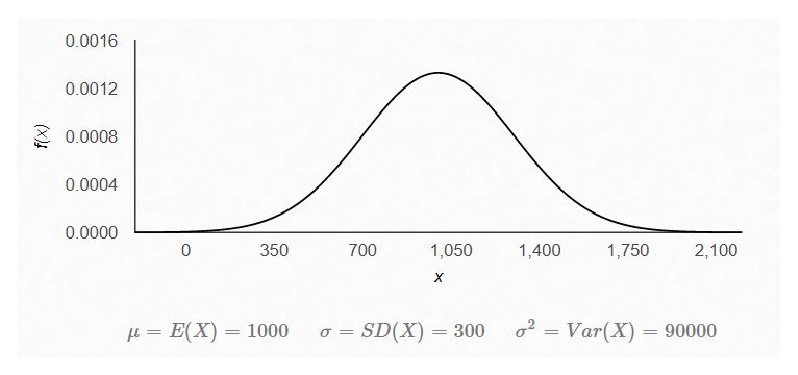
\epsfig{file = plsc43401_motivation_calculus_pic.eps, scale=.7}
\end{center}

\end{frame}


\begin{frame}
\frametitle{Example 2: Integral in Statistics }

\ \\Suppose that you get a very good score, say, 1500. \pause

\ \\A natural question to ask is: what's the probability of getting a score higher than 1500 in SAT test in 2018.

\ \\We need to compute this probability by: \pause

$$Pr(x \geq 1500) = \int_{1500}^{+ \infty} {\frac {1}{\sqrt {2\pi \sigma ^{2}}}}e^{-{\frac {(x-\mu )^{2}}{2\sigma ^{2}}}} dx = 0.04779$$
where $\sigma = 300$, $\mu = 1000$.

\end{frame}




\end{document}